\documentclass{beamer}
\usepackage[utf8]{inputenc}

\usetheme{Madrid}
\usecolortheme{default}
\usepackage{amsmath,amssymb,amsfonts,amsthm}
\usepackage{txfonts}
\usepackage{tkz-euclide}
\usepackage{listings}
\usepackage{adjustbox}
\usepackage{array}
\usepackage{tabularx}
\usepackage{gvv}
\usepackage{lmodern}
\usepackage{circuitikz}
\usepackage{tikz}
\usepackage{graphicx}

\setbeamertemplate{page number in head/foot}[totalframenumber]

\usepackage{tcolorbox}
\tcbuselibrary{minted,breakable,xparse,skins}



\definecolor{bg}{gray}{0.95}
\DeclareTCBListing{mintedbox}{O{}m!O{}}{%
  breakable=true,
  listing engine=minted,
  listing only,
  minted language=#2,
  minted style=default,
  minted options={%
    linenos,
    gobble=0,
    breaklines=true,
    breakafter=,,
    fontsize=\small,
    numbersep=8pt,
    #1},
  boxsep=0pt,
  left skip=0pt,
  right skip=0pt,
  left=25pt,
  right=0pt,
  top=3pt,
  bottom=3pt,
  arc=5pt,
  leftrule=0pt,
  rightrule=0pt,
  bottomrule=2pt,
  toprule=2pt,
  colback=bg,
  colframe=orange!70,
  enhanced,
  overlay={%
    \begin{tcbclipinterior}
    \fill[orange!20!white] (frame.south west) rectangle ([xshift=20pt]frame.north west);
    \end{tcbclipinterior}},
  #3,
}
\lstset{
    language=C,
    basicstyle=\ttfamily\small,
    keywordstyle=\color{blue},
    stringstyle=\color{orange},
    commentstyle=\color{green!60!black},
    numbers=left,
    numberstyle=\tiny\color{gray},
    breaklines=true,
    showstringspaces=false,
}
%------------------------------------------------------------
%This block of code defines the information to appear in the
%Title page
\title %optional
{2.4.41}
\date{August 31,2025}
%\subtitle{A short story}

\author % (optional)
{Sai Hasini Pappula-EE25BTECH11044}
\begin{document}

%----------------- Title -----------------
\begin{frame}
  \titlepage
\end{frame}

%----------------- Question -----------------
\begin{frame}{Question}
\begin{block}{Problem}
Determine whether the points 
$A(3,6,9), \; B(10,20,30), \; C(24,-41,5)$

are the vertices of a right-angled triangle using matrices.
\end{block}
\end{frame}

%----------------- Process Frame 1 -----------------
%----------------- Process Frame 1 -----------------
\begin{frame}{Process (Step 1)}
\textbf{Step 1: Represent points as vectors} \\
\begin{equation}
\myvec{A}=\begin{bmatrix}3\\6\\9\end{bmatrix}, \quad
\myvec{B}=\begin{bmatrix}10\\20\\30\end{bmatrix}, \quad
\myvec{C}=\begin{bmatrix}24\\-41\\5\end{bmatrix}
\end{equation}

\textbf{Step 2: Compute first difference vector} \\
\begin{equation}
\myvec{B}-\myvec{A} =
\begin{bmatrix}10-3\\20-6\\30-9\end{bmatrix} =
\begin{bmatrix}7\\14\\21\end{bmatrix}
\end{equation}
\end{frame}

%----------------- Process Frame 2 -----------------
\begin{frame}{Process (Step 2)}
\textbf{Step 2 (continued): Compute remaining difference vectors} \\
\begin{equation}
\myvec{C}-\myvec{B} =
\begin{bmatrix}24-10\\-41-20\\5-30\end{bmatrix} =
\begin{bmatrix}14\\-61\\-25\end{bmatrix}
\end{equation}

\begin{equation}
\myvec{C}-\myvec{A} =
\begin{bmatrix}24-3\\-41-6\\5-9\end{bmatrix} =
\begin{bmatrix}21\\-47\\-4\end{bmatrix}
\end{equation}

\textbf{Step 3: Use dot product test} \\
\begin{equation}
(\myvec{X}-\myvec{Y}) \cdot (\myvec{Z}-\myvec{W}) = 0 
\;\;\Rightarrow\;\; \text{Vectors are perpendicular}
\end{equation}
\end{frame}

%----------------- Final Answer -----------------
\begin{frame}{Conclusion}
Dot product results: \\
\begin{equation}
(\myvec{B}-\myvec{A}) \cdot (\myvec{C}-\myvec{A}) = -595
\end{equation}

\begin{equation}
(\myvec{B}-\myvec{A}) \cdot (\myvec{C}-\myvec{B}) = -1281
\end{equation}

\begin{equation}
(\myvec{C}-\myvec{A}) \cdot (\myvec{C}-\myvec{B}) = 3261
\end{equation}

Since none are zero, the points \textbf{do not form a right-angled triangle}.
\end{frame}



%----------------- C Code -----------------
\begin{frame}[fragile]{C Code}
\begin{lstlisting}[language=C]
#include <stdio.h>
int main() {
    double A[3] = {3, 6, 9};
    double B[3] = {10, 20, 30};
    double C[3] = {24, -41, 5};
    double dot1 = (B[0]-A[0])*(C[0]-A[0]) +
                  (B[1]-A[1])*(C[1]-A[1]) +
                  (B[2]-A[2])*(C[2]-A[2]);
    double dot2 = (B[0]-A[0])*(C[0]-B[0]) +
                  (B[1]-A[1])*(C[1]-B[1]) +
                  (B[2]-A[2])*(C[2]-B[2]);
    double dot3 = (C[0]-A[0])*(C[0]-B[0]) +
                  (C[1]-A[1])*(C[1]-B[1]) +
                  (C[2]-A[2])*(C[2]-B[2]);
    if(dot1==0 || dot2==0 || dot3==0)
        printf("Right-angled triangle\n");
    else
        printf("Not right-angled\n");
    return 0;
}
\end{lstlisting}
\end{frame}


%----------------- Python Code (Part 1) -----------------
\begin{frame}[fragile]{Python Code (1/2)}
\begin{lstlisting}[language=Python]
import numpy as np

A = np.array([3, 6, 9])
B = np.array([10, 20, 30])
C = np.array([24, -41, 5])

# Dot products computed directly
dot1 = np.dot(B-A, C-A)
dot2 = np.dot(B-A, C-B)
dot3 = np.dot(C-A, C-B)

if dot1 == 0 or dot2 == 0 or dot3 == 0:
    print("Right-angled triangle")
else:
    print("Not right-angled")
\end{lstlisting}
\end{frame}

%----------------- Python Code (Part 2) -----------------
\begin{frame}[fragile]{Python Code (2/2: Plot)}
\begin{lstlisting}[language=Python]
import matplotlib.pyplot as plt
from mpl_toolkits.mplot3d import Axes3D
fig = plt.figure(figsize=(8,6))
ax = fig.add_subplot(111, projection='3d')
ax.scatter(*A, color='black', s=80)
ax.text(A[0]+0.5, A[1]+0.5, A[2]+0.5, "A(3,6,9)")
ax.scatter(*B, color='blue', s=80)
ax.text(B[0]+0.5, B[1]+0.5, B[2]+0.5, "B(10,20,30)")

ax.scatter(*C, color='red', s=80)
ax.text(C[0]+0.5, C[1]+0.5, C[2]+0.5, "C(24,-41,5)")

ax.plot([A[0],B[0]], [A[1],B[1]], [A[2],B[2]], color='blue')
ax.plot([A[0],C[0]], [A[1],C[1]], [A[2],C[2]], color='green')
ax.plot([B[0],C[0]], [B[1],C[1]], [B[2],C[2]], color='red', linestyle='--')

plt.show()
\end{lstlisting}
\end{frame}


%----------------- Plot Image -----------------
\begin{frame}{Triangle in 3D}
\centering
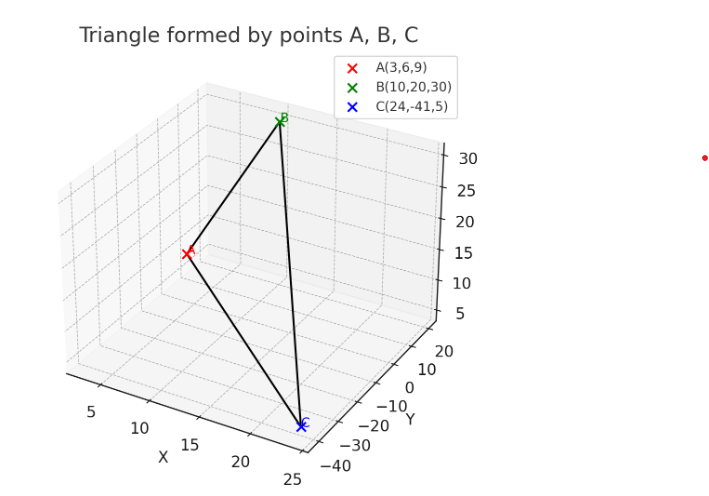
\includegraphics[width=0.7\columnwidth]{figs/plot3.png}
\end{frame}

\end{document}
